\chapter{Experiments}

In this chapter we discuss our experiments to evaluate performance of \ac{LVNMT} models with and without normalizing flows. We also consider settings to empirically evaluate the impact of latent variables on \ac{NMT} system. We include hyperparameter values in the supplement material, basing them off the work of \citet{eikema2018AEVNMT}. These hyperparameters were picked primarily with the generative \ac{LVNMT} system in mind, not the discriminative model. However, our main interest is not in the exact gains between models, and empirically these hyperparameters were sufficient.

To help prevent \textit{posterior collapse}, we perform KL-annealing linearly over the first 80,000 mini-batch updates. We choose a word-dropout rate of 0.1 for both models. Although , previous work suggested that word dropout is not necessarily help in the discriminative \ac{NMT} case \cite{harshil2018GNMT}. %\reminder{depending on performance of VNMT might move to doing the pretrained trick they describe}

We conducted our experiments with the IWSLT 2016 data sets available in the \textit{torchtext} library.\footnote{https://github.com/pytorch/text} We evaluated our models with the De-En language pair. This language pair was one we could more naturally evaluate subjectively.\footnote{ We did not do any formal human evaluation of translation quality.} We list total sentence counts in the supplement material. We evaluated performance with raw BLEU score with the library sacreBLEU \cite{post2018SacreBLEU}. For all experiments, we keep the random seed fixed to a single value for more fair evaluation of results. %, and note that these splits are from the ones available in Torch-Text library. \reminder{move last bit to supplement material, when you do add it also note that with the current TorchText we had to manually combine data as they do not do so with the current implementation}

We represented our vocabulary for each language with \ac{BPE} \cite{sennrich2015NMTRarwordsBPE}. We used vocabularies of 10,000 \ac{BPE}s per language. We found that larger vocabularies resulted in sub-word units that occurred infrequently enough to be uninformative from a practical learning perspective. We performed \ac{BPE} using the Sentence Piece library. \footnote{https://github.com/google/sentencepiece} We trained our \ac{NMT} models on sequences of maximum length 50. We translated sentences with beam search with 10 beams, and length normalization set to 1.0. Throughout our experiments we will refer to our discriminative models as \ac{VNMT} and our joint system as \ac{GNMT}. % The only other normalizing we did on our data sets was removing diacritics from the Arabic sentences. 


%Although most research in \ac{NMT} literature use beam search decoding, we choose to to use greedy decoding when translating sentences. Our general assumption is that if normalizing flows help with translation, this would carry over to heuristic searchers like beam search. Also, in recent literature studying the impact of beam search, larger beams do not necessarily translate to providing huge improvements in performance \cite{cohen2019unconstrained}. \reminder{ this...is a cop out midly because I saw performance degredation with my beam search algorithm set to 10... it worked fine on a 4,000,000 mil sentence dataset but that took waaaay to long}

%- Our networks use hidden layer sizes and embeddings of size 256 which is similar to the choices made in [eikeman et. al 2018] and we found for VNMT these parameters also worked better than those in [vnmt et. al.] for preliminary experiments on the WMT 2014 data they evaluated on. All specific params are in supplement material.
%We limit ourselves to these datasets, because it allows us to consider multiple language pairs and is a manageable size for our available computation budget. Due to these constraints, we caution readers that our results may not be applicable to datasets of different sizes.

\section{General Translation}

In this section we report our results when including normalizing flows on top of \ac{LVNMT} systems. Our hypothesis was that, given normalizing flows success in computer vision, that similar gains can be achieved by including normalizing flows in previously considered \ac{LVNMT} systems.  

Our baselines include the \ac{LVNMT} models we described in Chapter 3 with just the isotropic Gaussian distribution for the variational distribution. Our baselines optimize the \ac{ELBO} with the same number of \ac{MC} samples as our normalizing flows models to provide a fair comparison. This corresponds to better approximations of the negative log-likelihood of sequence predictions. The KL divergence is analytic in the Gaussian case which does not require sampling \cite{kingma2014autoencodingVB,rezende2014stochasticBackprop}. Although we do not report numbers, we did find just increasing the number of \ac{MC} samples improved translation quality on the validation set.

Table \ref{tab:de_en_besttranslations} shows the BLEU score of our results on the test set. The best model was picked based on validation BLEU score from checkpoints after every epoch of training. Each model was trained at least for 45 epochs.\footnote{When we say epoch we mean having updated on all sentence pairs before reshuffling mini-batches.} The boldfaced results represent the best performing version of a model for the given latent dimensions.

Overall, we found our generative model to perform better for any number of flows or latent space size. Even our worst performing generative model provide at least 1.0 BLEU score above the best performing discriminative model. This result is congruent with previous research suggesting joint learning is more effective than the simpler discriminative representation \cite{eikema2018AEVNMT}.

When considering latent dimensions of 128 and 256, we do find that normalizing flows can improve performance slightly based on BLEU score. These gains were more prominent in the discriminative modelling case as compared to the generative case. For \ac{VNMT}, even a single normalizing flow provided minute benefits. In contrast, \ac{GNMT} only saw performance gains with a latent space of 256, and even then only a few of the flows models outperformed the baseline. 

Our results seem to confirm previous findings on transform complexity, when comparing the flow type for a given number of flows for latent spaces 128 and 256. Generally the \ac{IAF} flows gave higher BLEU score with fewer flows compared to the same number of planar flows. This seems to affirm previous research showing that more complex flows require fewer layers to be beneficial \cite{kingma2016IAF,Berg2018SylvesterNF}. However, as we begin using higher numbers of flows we find that planar flows begin to perform marginally better. This would seem to highlight research suggesting better amortization schemes of flow parameters can generally be beneficial \cite{Berg2018SylvesterNF}, as well the limitations of planar flows transformation capabilities \cite{rezende2015VIwithNF,Berg2018SylvesterNF}.

The most surprising results was with our best overall model which had a latent space of 2. We originally considered such a small latent space for plotting purposes, but found it to be quite effective. Our findings would seem congruent with previous results on the value of smaller latent spaces \cite{schulz2018StochasticDecoder}. \footnote{We do not know if other researchers have also considered such small latent spaces. } Interestingly, our conclusions with flow complexity are reverse for this latent space where mostly planar flows perform better than \ac{IAF}. This would suggest for especially small latent spaces, that flexible transformations are more of a hindrance than beneficial to translation performance. 



\begin{table}[] 

	\caption{BLEU score for our models with normalizing flows for De-En translation. The best performing models are in bold for each type and number of flows. }
	\label{tab:de_en_besttranslations}

	\begin{tabular}{llllllll}
		\multicolumn{8}{c}{\textbf{Latent Dimension: 2}}                                                                                                                                                                                                                                                                                                                                                                                                                                                                                                        \\ \hline
		\multicolumn{1}{|l|}{\textbf{Flows}}                          & \multicolumn{1}{l|}{\textbf{1}}                              & \multicolumn{1}{l|}{\textbf{2}}                              & \multicolumn{1}{l|}{\textbf{4}}                             & \multicolumn{1}{l|}{\textbf{8}}                              & \multicolumn{1}{l|}{\textbf{16}}                             & \multicolumn{1}{l|}{\textbf{Baseline}}                                         & \multicolumn{1}{c|}{\textbf{Model}}                                          \\ \hline
		\rowcolor[HTML]{F9F9E1} 
		\multicolumn{1}{|l|}{\cellcolor[HTML]{F9F9E1}Planar}          & \multicolumn{1}{l|}{\cellcolor[HTML]{F9F9E1}\textbf{19.062}} & \multicolumn{1}{l|}{\cellcolor[HTML]{F9F9E1}18.949}          & \multicolumn{1}{l|}{\cellcolor[HTML]{F9F9E1}18.935}         & \multicolumn{1}{l|}{\cellcolor[HTML]{F9F9E1}19.009}          & \multicolumn{1}{l|}{\cellcolor[HTML]{F9F9E1}19.051}          & \multicolumn{1}{l|}{\cellcolor[HTML]{F9F9E1}}                                  & \multicolumn{1}{l|}{\cellcolor[HTML]{F9F9E1}}                                \\ \cline{1-6}
		\rowcolor[HTML]{F9F9E1} 
		\multicolumn{1}{|l|}{\cellcolor[HTML]{F9F9E1}IAF}             & \multicolumn{1}{l|}{\cellcolor[HTML]{F9F9E1}18.894}          & \multicolumn{1}{l|}{\cellcolor[HTML]{F9F9E1}18.477}          & \multicolumn{1}{l|}{\cellcolor[HTML]{F9F9E1}18.803}         & \multicolumn{1}{l|}{\cellcolor[HTML]{F9F9E1}\textbf{18.964}} & \multicolumn{1}{l|}{\cellcolor[HTML]{F9F9E1}18.67}           & \multicolumn{1}{l|}{\multirow{-2}{*}{\cellcolor[HTML]{F9F9E1}18.924}}          & \multicolumn{1}{l|}{\multirow{-2}{*}{\cellcolor[HTML]{F9F9E1}VNMT}}          \\ \hline
		\rowcolor[HTML]{F4DAD8} 
		\multicolumn{1}{|l|}{\cellcolor[HTML]{F4DAD8}Planar}          & \multicolumn{1}{l|}{\cellcolor[HTML]{F4DAD8}20.773}          & \multicolumn{1}{l|}{\cellcolor[HTML]{F4DAD8}20.696}          & \multicolumn{1}{l|}{\cellcolor[HTML]{F4DAD8}20.808}         & \multicolumn{1}{l|}{\cellcolor[HTML]{F4DAD8}20.863}          & \multicolumn{1}{l|}{\cellcolor[HTML]{F4DAD8}20.365}          & \multicolumn{1}{l|}{\cellcolor[HTML]{F4DAD8}}                                  & \multicolumn{1}{l|}{\cellcolor[HTML]{F4DAD8}}                                \\ \cline{1-6}
		\rowcolor[HTML]{F4DAD8} 
		\multicolumn{1}{|l|}{\cellcolor[HTML]{F4DAD8}IAF}             & \multicolumn{1}{l|}{\cellcolor[HTML]{F4DAD8}20.607}          & \multicolumn{1}{l|}{\cellcolor[HTML]{F4DAD8}20.515}          & \multicolumn{1}{l|}{\cellcolor[HTML]{F4DAD8}20.582}         & \multicolumn{1}{l|}{\cellcolor[HTML]{F4DAD8}20.552}          & \multicolumn{1}{l|}{\cellcolor[HTML]{F4DAD8}20.464}          & \multicolumn{1}{l|}{\multirow{-2}{*}{\cellcolor[HTML]{F4DAD8}\textbf{21.024}}} & \multicolumn{1}{l|}{\multirow{-2}{*}{\cellcolor[HTML]{F4DAD8}GNMT}}          \\ \hline
		\multicolumn{8}{c}{\textbf{Latent Dimension: 128}}                                                                                                                                                                                                                                                                                                                                                                                                                                                                                                      \\ \hline
		\multicolumn{1}{|l|}{\textbf{Flows}}                          & \multicolumn{1}{l|}{\textbf{1}}                              & \multicolumn{1}{l|}{\textbf{2}}                              & \multicolumn{1}{l|}{\textbf{4}}                             & \multicolumn{1}{l|}{\textbf{8}}                              & \multicolumn{1}{l|}{\textbf{16}}                             & \multicolumn{1}{l|}{\textbf{Baseline}}                                         & \multicolumn{1}{l|}{\textbf{Model}}                                          \\ \hline
		\rowcolor[HTML]{F9F9E1} 
		\multicolumn{1}{|l|}{\cellcolor[HTML]{F9F9E1}Planar}          & \multicolumn{1}{l|}{\cellcolor[HTML]{F9F9E1}18.843}          & \multicolumn{1}{l|}{\cellcolor[HTML]{F9F9E1}18.838}          & \multicolumn{1}{l|}{\cellcolor[HTML]{F9F9E1}19.139}         & \multicolumn{1}{l|}{\cellcolor[HTML]{F9F9E1}19.019}          & \multicolumn{1}{l|}{\cellcolor[HTML]{F9F9E1}\textbf{19.176}} & \multicolumn{1}{l|}{\cellcolor[HTML]{F9F9E1}}                                  & \multicolumn{1}{l|}{\cellcolor[HTML]{F9F9E1}}                                \\ \cline{1-6}
		\rowcolor[HTML]{F9F9E1} 
		\multicolumn{1}{|l|}{\cellcolor[HTML]{F9F9E1}IAF}             & \multicolumn{1}{l|}{\cellcolor[HTML]{F9F9E1}18.891}          & \multicolumn{1}{l|}{\cellcolor[HTML]{F9F9E1}18.957}          & \multicolumn{1}{l|}{\cellcolor[HTML]{F9F9E1}\textbf{19.29}} & \multicolumn{1}{l|}{\cellcolor[HTML]{F9F9E1}18.813}          & \multicolumn{1}{l|}{\cellcolor[HTML]{F9F9E1}18.92}           & \multicolumn{1}{l|}{\multirow{-2}{*}{\cellcolor[HTML]{F9F9E1}18.768}}          & \multicolumn{1}{l|}{\multirow{-2}{*}{\cellcolor[HTML]{F9F9E1}VNMT}}          \\ \hline
		\rowcolor[HTML]{F4DAD8} 
		\multicolumn{1}{|l|}{\cellcolor[HTML]{F4DAD8}Planar}          & \multicolumn{1}{l|}{\cellcolor[HTML]{F4DAD8}20.585}          & \multicolumn{1}{l|}{\cellcolor[HTML]{F4DAD8}20.595}          & \multicolumn{1}{l|}{\cellcolor[HTML]{F4DAD8}20.476}         & \multicolumn{1}{l|}{\cellcolor[HTML]{F4DAD8}20.553}          & \multicolumn{1}{l|}{\cellcolor[HTML]{F4DAD8}20.655}          & \multicolumn{1}{l|}{\cellcolor[HTML]{F4DAD8}}                                  & \multicolumn{1}{l|}{\cellcolor[HTML]{F4DAD8}}                                \\ \cline{1-6}
		\rowcolor[HTML]{F4DAD8} 
		\multicolumn{1}{|l|}{\cellcolor[HTML]{F4DAD8}IAF}             & \multicolumn{1}{l|}{\cellcolor[HTML]{F4DAD8}20.639}          & \multicolumn{1}{l|}{\cellcolor[HTML]{F4DAD8}20.64}           & \multicolumn{1}{l|}{\cellcolor[HTML]{F4DAD8}20.513}         & \multicolumn{1}{l|}{\cellcolor[HTML]{F4DAD8}20.646}          & \multicolumn{1}{l|}{\cellcolor[HTML]{F4DAD8}20.503}          & \multicolumn{1}{l|}{\multirow{-2}{*}{\cellcolor[HTML]{F4DAD8}\textbf{20.731}}} & \multicolumn{1}{l|}{\multirow{-2}{*}{\cellcolor[HTML]{F4DAD8}GNMT}}          \\ \hline
		\multicolumn{8}{c}{\textbf{Latent Dimension: 256}}                                                                                                                                                                                                                                                                                                                                                                                                                                                                                                      \\ \hline
		\multicolumn{1}{|l|}{\textbf{Flows}}                          & \multicolumn{1}{l|}{\textbf{1}}                              & \multicolumn{1}{l|}{\textbf{2}}                              & \multicolumn{1}{l|}{\textbf{4}}                             & \multicolumn{1}{l|}{\textbf{8}}                              & \multicolumn{1}{l|}{\textbf{16}}                             & \multicolumn{1}{l|}{\textbf{Baseline}}                                         & \multicolumn{1}{l|}{\textbf{Model}}                                          \\ \hline
		\rowcolor[HTML]{F9F9E1} 
		\multicolumn{1}{|l|}{\cellcolor[HTML]{F9F9E1}\textit{Planar}} & \multicolumn{1}{l|}{\cellcolor[HTML]{F9F9E1}18.934}          & \multicolumn{1}{l|}{\cellcolor[HTML]{F9F9E1}\textbf{19.263}} & \multicolumn{1}{l|}{\cellcolor[HTML]{F9F9E1}19.022}         & \multicolumn{1}{l|}{\cellcolor[HTML]{F9F9E1}18.79}           & \multicolumn{1}{l|}{\cellcolor[HTML]{F9F9E1}18.82}           & \multicolumn{1}{l|}{\cellcolor[HTML]{F9F9E1}}                                  & \multicolumn{1}{l|}{\cellcolor[HTML]{F9F9E1}}                                \\ \cline{1-6}
		\rowcolor[HTML]{F9F9E1} 
		\multicolumn{1}{|l|}{\cellcolor[HTML]{F9F9E1}\textit{IAF}}    & \multicolumn{1}{l|}{\cellcolor[HTML]{F9F9E1}18.953}          & \multicolumn{1}{l|}{\cellcolor[HTML]{F9F9E1}\textbf{19.173}} & \multicolumn{1}{l|}{\cellcolor[HTML]{F9F9E1}19.023}         & \multicolumn{1}{l|}{\cellcolor[HTML]{F9F9E1}18.986}          & \multicolumn{1}{l|}{\cellcolor[HTML]{F9F9E1}18.773}          & \multicolumn{1}{l|}{\multirow{-2}{*}{\cellcolor[HTML]{F9F9E1}18.761}}          & \multicolumn{1}{l|}{\multirow{-2}{*}{\cellcolor[HTML]{F9F9E1}\textit{VNMT}}} \\ \hline
		\rowcolor[HTML]{F4DAD8} 
		\multicolumn{1}{|l|}{\cellcolor[HTML]{F4DAD8}\textit{Planar}} & \multicolumn{1}{l|}{\cellcolor[HTML]{F4DAD8}20.551}          & \multicolumn{1}{l|}{\cellcolor[HTML]{F4DAD8}20.666}          & \multicolumn{1}{l|}{\cellcolor[HTML]{F4DAD8}20.537}         & \multicolumn{1}{l|}{\cellcolor[HTML]{F4DAD8}20.51}           & \multicolumn{1}{l|}{\cellcolor[HTML]{F4DAD8}\textbf{20.671}} & \multicolumn{1}{l|}{\cellcolor[HTML]{F4DAD8}}                                  & \multicolumn{1}{l|}{\cellcolor[HTML]{F4DAD8}}                                \\ \cline{1-6}
		\rowcolor[HTML]{F4DAD8} 
		\multicolumn{1}{|l|}{\cellcolor[HTML]{F4DAD8}\textit{IAF}}    & \multicolumn{1}{l|}{\cellcolor[HTML]{F4DAD8}20.85}           & \multicolumn{1}{l|}{\cellcolor[HTML]{F4DAD8}\textbf{20.864}} & \multicolumn{1}{l|}{\cellcolor[HTML]{F4DAD8}20.636}         & \multicolumn{1}{l|}{\cellcolor[HTML]{F4DAD8}20.619}          & \multicolumn{1}{l|}{\cellcolor[HTML]{F4DAD8}20.664}          & \multicolumn{1}{l|}{\multirow{-2}{*}{\cellcolor[HTML]{F4DAD8}20.655}}          & \multicolumn{1}{l|}{\multirow{-2}{*}{\cellcolor[HTML]{F4DAD8}\textit{GNMT}}} \\ \hline
	\end{tabular}
\end{table}

%For our baselines, we train both a VNMT and VAENMT model without normalizing flows. To provide equal comparisons we use the same number of samples as our normalizing flows models. In [Eqn for elbo] this corresponds to better approximations to the negative log-likelihood of sequence predictions as the KL divergence is analytic in the Gaussian case \cite{kingma, }. We consider latent dimensions of 2, 128 [best working latent space in Schulz et. al. 2018 for VNMT], and 256 [value used in Eikman et. al. model]. We consider latent dimensions of 2 as we plot the latent space with normalizing flows, and have previously seen this number of latent dimensions to perform quite well compared to large latent dimensions. We use a linear annealing schedule over the first 2 epochs of training to encourage both models to rely on the latent variables which has been shown to improve overall performance [cite cite cite]. We also try without any annealing to provide a comparison on gains from this annealing. We abstain from using word-dropout which is another regularization technique others have found useful previously to help with some models. Particularly in the VNMT case [GNMT paper] found that it did not help improve performance that particular system. 

%To evaluate our hypothesis, we then include normalizing flows on top of these existing systems keeping everything else in the system fixed. We again consider no annealing and annealing for 2 epochs, and train with N number of samples to approximate the ELBO during the training process. We consider 1, 2, 4, 8, and 16 flows to see if performance improves with an increasing number of flows. We test on the inverse autoregressive flows, and amortized planar flows available in the Pyro library. [might also consider Sylvester flows depending on the results from these...would require a smidge of implementing the amortization].

%We evaluate performance on the BLEU score and also measure the (-ELBO) and NLL during training to determine performance gains from normalizing flows. 




\section{Importance of Attention}

In this section, to see the utility of including latent variables, we train simplified version of our \ac{NMT} system which do not include the attention mechanism. Our motivation for this experiment is to see the impact of our latent variable as the only additional information to the decoding process. We do not expect this system to outperform the models with attention, particularly given the success of Transformer models \cite{vaswani2017attentionTransformer}. However, we hypothesize that if the latent variable can encode useful information in translation, then latent variables will still be better over systems without the latent variable. As an extension, normalizing flows will then enable these variables to be more beneficial by making the latent variable distribution more flexible.

Our modified models follow \citet{bahdanau2014NMTBYJoint} which means we include the latent variable in the generator network as a substitute for attention. In our previous experiment we did not consider this, as the focus was on incorporating normalizing flows in variations of existing models. We compare our modified discriminative model against a version of \citet{bahdanau2014NMTBYJoint} where attention is simply removed. In the joint modelling case, we use a baseline similar to the joint model of \citet{eikema2018AEVNMT} except without attention. Their model optimize the language model and translation systems separately except for sharing the source language word embeddings. All other hyperparameters are the same. Table \ref{tab:de_en_no_attention} show's results for our modified models and the baselines when evaluated with BLEU score. The best performing models are bold

Considering only the latent dimension size, we find an increase in performance simply doubling the dimensions of the latent variable. This would suggest that bigger latent spaces become more important when the model depends more on the latent variable. The combination of planar flows and \ac{VNMT} seem to benefit most from the latent variable, where as \ac{IAF} flows seem less effective. There could be several reasons, the most immediate conclusion being a bi-product of the random seed. One interpretation we suspect is related to the \ac{IAF}s design of compared to planar flows. As our \ac{GRU}s are fairly small compared to other models, and sensitive to small perturbations, they cannot as well utilize these more complex distributions. Another might be that as our planar flows provide per-sentence flow parameters, making them more flexible. In comparison, the \ac{IAF} is unable to capture this more nuance information by simply conditioning on a context vector. 

 Unfortunately, our \ac{GNMT} model did not benefit from the inclusion of normalizing flows and was actually hindered in performance for most choices of flows. We reason this is due to the formulation of \ac{GNMT}. The latent variable initialize the translation system beginning in the encoder network as compared to being passed as input during decoding. This means, our decoder never actually see the latent variable directly. Without this explicit information, the model is relying on the \ac{GRU}s to implicitly keep this information from beginning to end which, based on our results is less effective than the input feeding approach of \ac{VNMT} to benefit from normalizing flows. 


\begin{table}[]
	\caption{Results for translation systems without attention mechanism. Baseline are deterministic version of models excluding latent variables.}
	\label{tab:de_en_no_attention}
\begin{tabular}{lllllllll}
	\multicolumn{9}{c}{\textbf{Latent Dimension: 128}}                                                                                                                                                                                                                                                                                                                                                                                                                                                                                                                                                      \\ \hline
	\multicolumn{1}{|l|}{\textbf{Flows}}                          & \multicolumn{1}{c|}{\textbf{0}}                                               & \multicolumn{1}{c|}{\textbf{1}}                             & \multicolumn{1}{c|}{\textbf{2}}                    & \multicolumn{1}{c|}{\textbf{4}}                    & \multicolumn{1}{c|}{\textbf{8}}                             & \multicolumn{1}{c|}{\textbf{16}}                            & \multicolumn{1}{l|}{\textbf{Baseline}}                               & \multicolumn{1}{l|}{\textbf{Model}}                                          \\ \hline
	\rowcolor[HTML]{F9F9E1} 
	\multicolumn{1}{|l|}{\cellcolor[HTML]{F9F9E1}Planar}          & \multicolumn{1}{l|}{\cellcolor[HTML]{F9F9E1}}                                 & \multicolumn{1}{l|}{\cellcolor[HTML]{F9F9E1}6.61}           & \multicolumn{1}{l|}{\cellcolor[HTML]{F9F9E1}6.637} & \multicolumn{1}{l|}{\cellcolor[HTML]{F9F9E1}6.626} & \multicolumn{1}{l|}{\cellcolor[HTML]{F9F9E1}\textbf{6.931}} & \multicolumn{1}{l|}{\cellcolor[HTML]{F9F9E1}6.782}          & \multicolumn{1}{l|}{\cellcolor[HTML]{F9F9E1}}                        & \multicolumn{1}{l|}{\cellcolor[HTML]{F9F9E1}}                                \\ \cline{1-1} \cline{3-7}
	\rowcolor[HTML]{F9F9E1} 
	\multicolumn{1}{|l|}{\cellcolor[HTML]{F9F9E1}IAF}             & \multicolumn{1}{l|}{\multirow{-2}{*}{\cellcolor[HTML]{F9F9E1}6.249}}          & \multicolumn{1}{l|}{\cellcolor[HTML]{F9F9E1}\textbf{6.417}} & \multicolumn{1}{l|}{\cellcolor[HTML]{F9F9E1}6.321} & \multicolumn{1}{l|}{\cellcolor[HTML]{F9F9E1}6.278} & \multicolumn{1}{l|}{\cellcolor[HTML]{F9F9E1}5.983}          & \multicolumn{1}{l|}{\cellcolor[HTML]{F9F9E1}5.918}          & \multicolumn{1}{l|}{\multirow{-2}{*}{\cellcolor[HTML]{F9F9E1}6.383}} & \multicolumn{1}{l|}{\multirow{-2}{*}{\cellcolor[HTML]{F9F9E1}VNMT}}          \\ \hline
	\rowcolor[HTML]{F4DAD8} 
	\multicolumn{1}{|l|}{\cellcolor[HTML]{F4DAD8}Planar}          & \multicolumn{1}{l|}{\cellcolor[HTML]{F4DAD8}\textbf{7.365}}                   & \multicolumn{1}{l|}{\cellcolor[HTML]{F4DAD8}7.2}            & \multicolumn{1}{l|}{\cellcolor[HTML]{F4DAD8}7.217} & \multicolumn{1}{l|}{\cellcolor[HTML]{F4DAD8}7.19}  & \multicolumn{1}{l|}{\cellcolor[HTML]{F4DAD8}7.105}          & \multicolumn{1}{l|}{\cellcolor[HTML]{F4DAD8}7.246}          & \multicolumn{1}{l|}{\cellcolor[HTML]{F4DAD8}}                        & \multicolumn{1}{l|}{\cellcolor[HTML]{F4DAD8}}                                \\ \cline{1-7}
	\rowcolor[HTML]{F4DAD8} 
	\multicolumn{1}{|l|}{\cellcolor[HTML]{F4DAD8}IAF}             & \multicolumn{1}{l|}{\cellcolor[HTML]{F4DAD8}7.365}                            & \multicolumn{1}{l|}{\cellcolor[HTML]{F4DAD8}7.314}          & \multicolumn{1}{l|}{\cellcolor[HTML]{F4DAD8}7.371} & \multicolumn{1}{l|}{\cellcolor[HTML]{F4DAD8}7.325} & \multicolumn{1}{l|}{\cellcolor[HTML]{F4DAD8}7.182}          & \multicolumn{1}{l|}{\cellcolor[HTML]{F4DAD8}\textbf{7.413}} & \multicolumn{1}{l|}{\multirow{-2}{*}{\cellcolor[HTML]{F4DAD8}6.289}}  & \multicolumn{1}{l|}{\multirow{-2}{*}{\cellcolor[HTML]{F4DAD8}GNMT}}          \\ \hline
	\multicolumn{9}{c}{\textbf{Latent Dimension: 256}}                                                                                                                                                                                                                                                                                                                                                                                                                                                                                                                                                      \\ \hline
	\multicolumn{1}{|l|}{\textbf{Flows}}                          & \multicolumn{1}{c|}{\textbf{0}}                                               & \multicolumn{1}{c|}{\textbf{1}}                             & \multicolumn{1}{c|}{\textbf{2}}                    & \multicolumn{1}{c|}{\textbf{4}}                    & \multicolumn{1}{c|}{\textbf{8}}                             & \multicolumn{1}{c|}{\textbf{16}}                            & \multicolumn{1}{l|}{\textbf{Baseline}}                               & \multicolumn{1}{l|}{\textbf{Model}}                                          \\ \hline
	\rowcolor[HTML]{F9F9E1} 
	\multicolumn{1}{|l|}{\cellcolor[HTML]{F9F9E1}\textit{Planar}} & \multicolumn{1}{l|}{\cellcolor[HTML]{F9F9E1}}                                 & \multicolumn{1}{l|}{\cellcolor[HTML]{F9F9E1}6.307}          & \multicolumn{1}{l|}{\cellcolor[HTML]{F9F9E1}6.813} & \multicolumn{1}{l|}{\cellcolor[HTML]{F9F9E1}6.911} & \multicolumn{1}{l|}{\cellcolor[HTML]{F9F9E1}7.371}          & \multicolumn{1}{l|}{\cellcolor[HTML]{F9F9E1}\textbf{7.383}} & \multicolumn{1}{l|}{\cellcolor[HTML]{F9F9E1}}                        & \multicolumn{1}{l|}{\cellcolor[HTML]{F9F9E1}}                                \\ \cline{1-1} \cline{3-7}
	\rowcolor[HTML]{F9F9E1} 
	\multicolumn{1}{|l|}{\cellcolor[HTML]{F9F9E1}\textit{IAF}}    & \multicolumn{1}{l|}{\multirow{-2}{*}{\cellcolor[HTML]{F9F9E1}6.432}}          & \multicolumn{1}{l|}{\cellcolor[HTML]{F9F9E1}6.452}          & \multicolumn{1}{l|}{\cellcolor[HTML]{F9F9E1}6.474} & \multicolumn{1}{l|}{\cellcolor[HTML]{F9F9E1}6.4}   & \multicolumn{1}{l|}{\cellcolor[HTML]{F9F9E1}6.226}          & \multicolumn{1}{l|}{\cellcolor[HTML]{F9F9E1}\textbf{6.708}} & \multicolumn{1}{l|}{\multirow{-2}{*}{\cellcolor[HTML]{F9F9E1}6.383}} & \multicolumn{1}{l|}{\multirow{-2}{*}{\cellcolor[HTML]{F9F9E1}\textit{VNMT}}} \\ \hline
	\rowcolor[HTML]{F4DAD8} 
	\multicolumn{1}{|l|}{\cellcolor[HTML]{F4DAD8}\textit{Planar}} & \multicolumn{1}{l|}{\cellcolor[HTML]{F4DAD8}}                                 & \multicolumn{1}{l|}{\cellcolor[HTML]{F4DAD8}7.398}          & \multicolumn{1}{l|}{\cellcolor[HTML]{F4DAD8}7.217} & \multicolumn{1}{l|}{\cellcolor[HTML]{F4DAD8}7.332} & \multicolumn{1}{l|}{\cellcolor[HTML]{F4DAD8}7.262}          & \multicolumn{1}{l|}{\cellcolor[HTML]{F4DAD8}7.074}          & \multicolumn{1}{l|}{\cellcolor[HTML]{F4DAD8}}                        & \multicolumn{1}{l|}{\cellcolor[HTML]{F4DAD8}}                                \\ \cline{1-1} \cline{3-7}
	\rowcolor[HTML]{F4DAD8} 
	\multicolumn{1}{|l|}{\cellcolor[HTML]{F4DAD8}\textit{IAF}}    & \multicolumn{1}{l|}{\multirow{-2}{*}{\cellcolor[HTML]{F4DAD8}\textbf{7.505}}} & \multicolumn{1}{l|}{\cellcolor[HTML]{F4DAD8}7.349}          & \multicolumn{1}{l|}{\cellcolor[HTML]{F4DAD8}7.344} & \multicolumn{1}{l|}{\cellcolor[HTML]{F4DAD8}7.278} & \multicolumn{1}{l|}{\cellcolor[HTML]{F4DAD8}7.04}           & \multicolumn{1}{l|}{\cellcolor[HTML]{F4DAD8}7.359}          & \multicolumn{1}{l|}{\multirow{-2}{*}{\cellcolor[HTML]{F4DAD8} 6.289}}  & \multicolumn{1}{l|}{\multirow{-2}{*}{\cellcolor[HTML]{F4DAD8}\textit{GNMT}}} \\ \hline
\end{tabular}
\end{table}

\section{Value of Latent Variable} 

%Hypothesis: If the latent variable is encoding information important to the translation process, it stands to reason setting Z = [0, 0 ,.... 0] during the evaluation process will negatively impact translation performance, as otherwise the latent variable z is not encoding useful information in the system.

%Previous research which incorporate latent variables in \ac{NMT} systems have often focused on non-zero KL values as justification for the latent variable encoding information for the generative system. The argument in favor of this metric is that the magnitude of the KL can be used a heuristic to gauge the importance the latent variable plays in the translation system. This stems from the fact that typically the prior is a stationary target and if the KL term is small that the latent variable is uninformative to the system's performance. A limitation of this measurement is that it is not applicable in situation where the prior is learned jointly, such as in our \ac{VNMT} system.

In previous works, the utility of latent variables is typically justified by training a similar system without the latent variable included, or being optimized differently.  In cases where the prior is stationary, authors then typically report the KL divergence to justify the latent variables usage. This metric is inapplicable to \ac{VNMT} where the prior is learned. In the ideal \ac{VNMT} scenario, the KL divergence being 0 indicating both distributions encode the same information.

As an alternative approach to measure the value of our latent variable during translation, we set Z to the 0 vector. We measure the difference in BLEU score with and without Z during the decoding process. This can give us direct insight into the importance of Z when translating sentences, whether the prior is learned or not. Table \ref{tab:de_en_kl_divergence} provides the Kl divergence and \ref{tab:de_en_delta_bleu} show the difference in BLEU score when Z is the 0 vector. 

Interestingly, for many of our \ac{VNMT} models with planar flows we see including $Z$ often negatively impacts performance of the translation system. This could suggest that the latent variable itself is not helping the translation, but improves representations in the encoder or source word embeddings. Another explanation is that our substitution of $p_{\theta}$ for $q_{\phi}$ at decode time provide information that is too dissimilar to the variational distribution. This is plausible given that in many cases the KL divergence is non 0, but even in several instances a lower KL divergence still lead to loss of performance with Z. These substitution approaches have also previously been shown to provide minimal or mixed results in terms of comparative performances \cite{eikema2018AEVNMT}.

The exception to our above observations of course is our \ac{VNMT} with \ac{IAF} models in higher dimensions which seem to heavily depend on the latent variable. One possible reason for this has to do with the amortization of \ac{IAF} flows. As these flows are composed of neural networks shared across data points, they can more easily be viewed as additional layers in the network. In a similar setting, one bug we found in our implementation was excluding the projection layer and found similar performance drops to those with out IAF flows results. This could also be a more volatile result which occurs due to different choices of initialization. It has been noted KL annealing schemes can be sensitive to final performance in this regard \cite{sphericallatent2018Xu}.

In comparison, \ac{GNMT} seems to generally show at least minute dependence on the latent variable regardless of number of flows. There do not seem to be any clear patterns between choices about flows and the information encoded by $z$. Likewise, a higher KL divergence does not necessarily correspond with more utility in translation performance.  

In comparison, when we perform the same experiment with our \ac{LVNMT} systems without attention, we see more dependence on the latent variable. Our results are in table \ref{tab:de_en_no_attention_delta_bleu} and \ref{tab:de_en_no_attention_kl_div}. In most cases with planar flows, we see our models depend more on the latent variable as opposed to without the system. Our \ac{IAF} flows models are more mixed in terms of performance changes, where in \ac{GNMT} our models depend more on the flows with a smaller latent dimension space as opposed to larger latent space. 



\begin{table}
	\caption{Average KL divergence for the test set. For \ac{VNMT} the KL term should be smaller meaning the distributions encoder similar information. for \ac{GNMT} they should be higher as these suggest more informative latent spaces.  }
	\label{tab:de_en_kl_divergence}
	\begin{tabular}{llllllll}
		\multicolumn{8}{c}{\textbf{Latent Dimension: 2 (KL Difference)}}                                                                                                                                                                                                                                                                                                                                                                                                                              \\ \hline
		\multicolumn{1}{|l|}{\textbf{Flows}}                          & \multicolumn{1}{l|}{\textbf{1}}                    & \multicolumn{1}{l|}{\textbf{2}}                    & \multicolumn{1}{l|}{\textbf{4}}                     & \multicolumn{1}{l|}{\textbf{8}}                    & \multicolumn{1}{l|}{\textbf{16}}                   & \multicolumn{1}{l|}{\textbf{Baseline}}                               & \multicolumn{1}{c|}{\textbf{Model}}                                          \\ \hline
		\rowcolor[HTML]{F9F9E1} 
		\multicolumn{1}{|l|}{\cellcolor[HTML]{F9F9E1}Planar}          & \multicolumn{1}{l|}{\cellcolor[HTML]{F9F9E1}0.94}  & \multicolumn{1}{l|}{\cellcolor[HTML]{F9F9E1}1.446} & \multicolumn{1}{l|}{\cellcolor[HTML]{F9F9E1}0.679}  & \multicolumn{1}{l|}{\cellcolor[HTML]{F9F9E1}0}     & \multicolumn{1}{l|}{\cellcolor[HTML]{F9F9E1}0}     & \multicolumn{1}{l|}{\cellcolor[HTML]{F9F9E1}}                        & \multicolumn{1}{l|}{\cellcolor[HTML]{F9F9E1}}                                \\ \cline{1-6}
		\rowcolor[HTML]{F9F9E1} 
		\multicolumn{1}{|l|}{\cellcolor[HTML]{F9F9E1}IAF}             & \multicolumn{1}{l|}{\cellcolor[HTML]{F9F9E1}1.15}  & \multicolumn{1}{l|}{\cellcolor[HTML]{F9F9E1}1.564} & \multicolumn{1}{l|}{\cellcolor[HTML]{F9F9E1}1.395}  & \multicolumn{1}{l|}{\cellcolor[HTML]{F9F9E1}0.846} & \multicolumn{1}{l|}{\cellcolor[HTML]{F9F9E1}1.559} & \multicolumn{1}{l|}{\multirow{-2}{*}{\cellcolor[HTML]{F9F9E1}1.154}} & \multicolumn{1}{l|}{\multirow{-2}{*}{\cellcolor[HTML]{F9F9E1}VNMT}}          \\ \hline
		\rowcolor[HTML]{F4DAD8} 
		\multicolumn{1}{|l|}{\cellcolor[HTML]{F4DAD8}Planar}          & \multicolumn{1}{l|}{\cellcolor[HTML]{F4DAD8}2.481} & \multicolumn{1}{l|}{\cellcolor[HTML]{F4DAD8}2.319} & \multicolumn{1}{l|}{\cellcolor[HTML]{F4DAD8}2.005}  & \multicolumn{1}{l|}{\cellcolor[HTML]{F4DAD8}0.104} & \multicolumn{1}{l|}{\cellcolor[HTML]{F4DAD8}3.661} & \multicolumn{1}{l|}{\cellcolor[HTML]{F4DAD8}}                        & \multicolumn{1}{l|}{\cellcolor[HTML]{F4DAD8}}                                \\ \cline{1-6}
		\rowcolor[HTML]{F4DAD8} 
		\multicolumn{1}{|l|}{\cellcolor[HTML]{F4DAD8}IAF}             & \multicolumn{1}{l|}{\cellcolor[HTML]{F4DAD8}0}     & \multicolumn{1}{l|}{\cellcolor[HTML]{F4DAD8}2.362} & \multicolumn{1}{l|}{\cellcolor[HTML]{F4DAD8}3.913}  & \multicolumn{1}{l|}{\cellcolor[HTML]{F4DAD8}2.086} & \multicolumn{1}{l|}{\cellcolor[HTML]{F4DAD8}2.625} & \multicolumn{1}{l|}{\multirow{-2}{*}{\cellcolor[HTML]{F4DAD8}2.992}} & \multicolumn{1}{l|}{\multirow{-2}{*}{\cellcolor[HTML]{F4DAD8}GNMT}}          \\ \hline
		\multicolumn{8}{c}{\textbf{Latent Dimension: 128}}                                                                                                                                                                                                                                                                                                                                                                                                                                            \\ \hline
		\multicolumn{1}{|l|}{\textbf{Flows}}                          & \multicolumn{1}{l|}{\textbf{1}}                    & \multicolumn{1}{l|}{\textbf{2}}                    & \multicolumn{1}{l|}{\textbf{4}}                     & \multicolumn{1}{l|}{\textbf{8}}                    & \multicolumn{1}{l|}{\textbf{16}}                   & \multicolumn{1}{l|}{\textbf{Baseline}}                               & \multicolumn{1}{l|}{\textbf{Model}}                                          \\ \hline
		\rowcolor[HTML]{F9F9E1} 
		\multicolumn{1}{|l|}{\cellcolor[HTML]{F9F9E1}Planar}          & \multicolumn{1}{l|}{\cellcolor[HTML]{F9F9E1}2.157} & \multicolumn{1}{l|}{\cellcolor[HTML]{F9F9E1}1.269} & \multicolumn{1}{l|}{\cellcolor[HTML]{F9F9E1}1.181}  & \multicolumn{1}{l|}{\cellcolor[HTML]{F9F9E1}1.037} & \multicolumn{1}{l|}{\cellcolor[HTML]{F9F9E1}1.625} & \multicolumn{1}{l|}{\cellcolor[HTML]{F9F9E1}}                        & \multicolumn{1}{l|}{\cellcolor[HTML]{F9F9E1}}                                \\ \cline{1-6}
		\rowcolor[HTML]{F9F9E1} 
		\multicolumn{1}{|l|}{\cellcolor[HTML]{F9F9E1}IAF}             & \multicolumn{1}{l|}{\cellcolor[HTML]{F9F9E1}0.682} & \multicolumn{1}{l|}{\cellcolor[HTML]{F9F9E1}1.346} & \multicolumn{1}{l|}{\cellcolor[HTML]{F9F9E1}1.318}  & \multicolumn{1}{l|}{\cellcolor[HTML]{F9F9E1}1.595} & \multicolumn{1}{l|}{\cellcolor[HTML]{F9F9E1}1.059} & \multicolumn{1}{l|}{\multirow{-2}{*}{\cellcolor[HTML]{F9F9E1}1.039}} & \multicolumn{1}{l|}{\multirow{-2}{*}{\cellcolor[HTML]{F9F9E1}VNMT}}          \\ \hline
		\rowcolor[HTML]{F4DAD8} 
		\multicolumn{1}{|l|}{\cellcolor[HTML]{F4DAD8}Planar}          & \multicolumn{1}{l|}{\cellcolor[HTML]{F4DAD8}3.226} & \multicolumn{1}{l|}{\cellcolor[HTML]{F4DAD8}3.154} & \multicolumn{1}{l|}{\cellcolor[HTML]{F4DAD8}2.356}  & \multicolumn{1}{l|}{\cellcolor[HTML]{F4DAD8}2.824} & \multicolumn{1}{l|}{\cellcolor[HTML]{F4DAD8}3.644} & \multicolumn{1}{l|}{\cellcolor[HTML]{F4DAD8}}                        & \multicolumn{1}{l|}{\cellcolor[HTML]{F4DAD8}}                                \\ \cline{1-6}
		\rowcolor[HTML]{F4DAD8} 
		\multicolumn{1}{|l|}{\cellcolor[HTML]{F4DAD8}IAF}             & \multicolumn{1}{l|}{\cellcolor[HTML]{F4DAD8}4.308} & \multicolumn{1}{l|}{\cellcolor[HTML]{F4DAD8}4.356} & \multicolumn{1}{l|}{\cellcolor[HTML]{F4DAD8}4.185}  & \multicolumn{1}{l|}{\cellcolor[HTML]{F4DAD8}4.432} & \multicolumn{1}{l|}{\cellcolor[HTML]{F4DAD8}4.141} & \multicolumn{1}{l|}{\multirow{-2}{*}{\cellcolor[HTML]{F4DAD8}4.394}} & \multicolumn{1}{l|}{\multirow{-2}{*}{\cellcolor[HTML]{F4DAD8}GNMT}}          \\ \hline
		\multicolumn{8}{c}{\textbf{Latent Dimension: 256}}                                                                                                                                                                                                                                                                                                                                                                                                                                            \\ \hline
		\multicolumn{1}{|l|}{\textbf{Flows}}                          & \multicolumn{1}{l|}{\textbf{1}}                    & \multicolumn{1}{l|}{\textbf{2}}                    & \multicolumn{1}{l|}{\textbf{4}}                     & \multicolumn{1}{l|}{\textbf{8}}                    & \multicolumn{1}{l|}{\textbf{16}}                   & \multicolumn{1}{l|}{\textbf{Baseline}}                               & \multicolumn{1}{l|}{\textbf{Model}}                                          \\ \hline
		\rowcolor[HTML]{F9F9E1} 
		\multicolumn{1}{|l|}{\cellcolor[HTML]{F9F9E1}\textit{Planar}} & \multicolumn{1}{l|}{\cellcolor[HTML]{F9F9E1}0.917} & \multicolumn{1}{l|}{\cellcolor[HTML]{F9F9E1}2.352} & \multicolumn{1}{l|}{\cellcolor[HTML]{F9F9E1}2.372}  & \multicolumn{1}{l|}{\cellcolor[HTML]{F9F9E1}1.112} & \multicolumn{1}{l|}{\cellcolor[HTML]{F9F9E1}1.266} & \multicolumn{1}{l|}{\cellcolor[HTML]{F9F9E1}}                        & \multicolumn{1}{l|}{\cellcolor[HTML]{F9F9E1}}                                \\ \cline{1-6}
		\rowcolor[HTML]{F9F9E1} 
		\multicolumn{1}{|l|}{\cellcolor[HTML]{F9F9E1}\textit{IAF}}    & \multicolumn{1}{l|}{\cellcolor[HTML]{F9F9E1}2.414} & \multicolumn{1}{l|}{\cellcolor[HTML]{F9F9E1}1.935} & \multicolumn{1}{l|}{\cellcolor[HTML]{F9F9E1}1.143}  & \multicolumn{1}{l|}{\cellcolor[HTML]{F9F9E1}1.1}   & \multicolumn{1}{l|}{\cellcolor[HTML]{F9F9E1}1.099} & \multicolumn{1}{l|}{\multirow{-2}{*}{\cellcolor[HTML]{F9F9E1}1.995}} & \multicolumn{1}{l|}{\multirow{-2}{*}{\cellcolor[HTML]{F9F9E1}\textit{VNMT}}} \\ \hline
		\rowcolor[HTML]{F4DAD8} 
		\multicolumn{1}{|l|}{\cellcolor[HTML]{F4DAD8}\textit{Planar}} & \multicolumn{1}{l|}{\cellcolor[HTML]{F4DAD8}4.337} & \multicolumn{1}{l|}{\cellcolor[HTML]{F4DAD8}3.93}  & \multicolumn{1}{l|}{\cellcolor[HTML]{F4DAD8}16.144} & \multicolumn{1}{l|}{\cellcolor[HTML]{F4DAD8}2.749} & \multicolumn{1}{l|}{\cellcolor[HTML]{F4DAD8}17.44} & \multicolumn{1}{l|}{\cellcolor[HTML]{F4DAD8}}                        & \multicolumn{1}{l|}{\cellcolor[HTML]{F4DAD8}}                                \\ \cline{1-6}
		\rowcolor[HTML]{F4DAD8} 
		\multicolumn{1}{|l|}{\cellcolor[HTML]{F4DAD8}\textit{IAF}}    & \multicolumn{1}{l|}{\cellcolor[HTML]{F4DAD8}3.866} & \multicolumn{1}{l|}{\cellcolor[HTML]{F4DAD8}3.742} & \multicolumn{1}{l|}{\cellcolor[HTML]{F4DAD8}3.998}  & \multicolumn{1}{l|}{\cellcolor[HTML]{F4DAD8}3.985} & \multicolumn{1}{l|}{\cellcolor[HTML]{F4DAD8}3.98}  & \multicolumn{1}{l|}{\multirow{-2}{*}{\cellcolor[HTML]{F4DAD8}3.838}} & \multicolumn{1}{l|}{\multirow{-2}{*}{\cellcolor[HTML]{F4DAD8}\textit{GNMT}}} \\ \hline
	\end{tabular}
\end{table}


\begin{table}[]
	\caption{Change in BLEU score when Z is set to 0 vector at decode time. Negative numbers indicate our models do better without Z included during translation.}
	\label{tab:de_en_delta_bleu}
	\begin{tabular}{llllllll}
		\multicolumn{8}{c}{\textbf{Latent Dimension: 2 (BLEU difference)}}                                                                                                                                                                                                                                                                                                                                                                                                                                 \\ \hline
		\multicolumn{1}{|l|}{\textbf{Flows}}                          & \multicolumn{1}{l|}{\textbf{1}}                     & \multicolumn{1}{l|}{\textbf{2}}                     & \multicolumn{1}{l|}{\textbf{4}}                     & \multicolumn{1}{l|}{\textbf{8}}                     & \multicolumn{1}{l|}{\textbf{16}}                    & \multicolumn{1}{l|}{\textbf{Baseline}}                                & \multicolumn{1}{c|}{\textbf{Model}}                                          \\ \hline
		\rowcolor[HTML]{F9F9E1} 
		\multicolumn{1}{|l|}{\cellcolor[HTML]{F9F9E1}Planar}          & \multicolumn{1}{l|}{\cellcolor[HTML]{F9F9E1}0.003}  & \multicolumn{1}{l|}{\cellcolor[HTML]{F9F9E1}-0.094} & \multicolumn{1}{l|}{\cellcolor[HTML]{F9F9E1}-0.06}  & \multicolumn{1}{l|}{\cellcolor[HTML]{F9F9E1}0.04}   & \multicolumn{1}{l|}{\cellcolor[HTML]{F9F9E1}-0.003} & \multicolumn{1}{l|}{\cellcolor[HTML]{F9F9E1}}                         & \multicolumn{1}{l|}{\cellcolor[HTML]{F9F9E1}}                                \\ \cline{1-6}
		\rowcolor[HTML]{F9F9E1} 
		\multicolumn{1}{|l|}{\cellcolor[HTML]{F9F9E1}IAF}             & \multicolumn{1}{l|}{\cellcolor[HTML]{F9F9E1}-0.008} & \multicolumn{1}{l|}{\cellcolor[HTML]{F9F9E1}0.058}  & \multicolumn{1}{l|}{\cellcolor[HTML]{F9F9E1}-0.102} & \multicolumn{1}{l|}{\cellcolor[HTML]{F9F9E1}-0.102} & \multicolumn{1}{l|}{\cellcolor[HTML]{F9F9E1}-0.114} & \multicolumn{1}{l|}{\multirow{-2}{*}{\cellcolor[HTML]{F9F9E1}-0.102}} & \multicolumn{1}{l|}{\multirow{-2}{*}{\cellcolor[HTML]{F9F9E1}VNMT}}          \\ \hline
		\rowcolor[HTML]{F4DAD8} 
		\multicolumn{1}{|l|}{\cellcolor[HTML]{F4DAD8}Planar}          & \multicolumn{1}{l|}{\cellcolor[HTML]{F4DAD8}0.246}  & \multicolumn{1}{l|}{\cellcolor[HTML]{F4DAD8}-0.027} & \multicolumn{1}{l|}{\cellcolor[HTML]{F4DAD8}0.109}  & \multicolumn{1}{l|}{\cellcolor[HTML]{F4DAD8}0.036}  & \multicolumn{1}{l|}{\cellcolor[HTML]{F4DAD8}0.226}  & \multicolumn{1}{l|}{\cellcolor[HTML]{F4DAD8}}                         & \multicolumn{1}{l|}{\cellcolor[HTML]{F4DAD8}}                                \\ \cline{1-6}
		\rowcolor[HTML]{F4DAD8} 
		\multicolumn{1}{|l|}{\cellcolor[HTML]{F4DAD8}IAF}             & \multicolumn{1}{l|}{\cellcolor[HTML]{F4DAD8}0.003}  & \multicolumn{1}{l|}{\cellcolor[HTML]{F4DAD8}0.109}  & \multicolumn{1}{l|}{\cellcolor[HTML]{F4DAD8}0.005}  & \multicolumn{1}{l|}{\cellcolor[HTML]{F4DAD8}0.1}    & \multicolumn{1}{l|}{\cellcolor[HTML]{F4DAD8}-0.023} & \multicolumn{1}{l|}{\multirow{-2}{*}{\cellcolor[HTML]{F4DAD8}0.239}}  & \multicolumn{1}{l|}{\multirow{-2}{*}{\cellcolor[HTML]{F4DAD8}GNMT}}          \\ \hline
		\multicolumn{8}{c}{\textbf{Latent Dimension: 128}}                                                                                                                                                                                                                                                                                                                                                                                                                                                 \\ \hline
		\multicolumn{1}{|l|}{\textbf{Flows}}                          & \multicolumn{1}{l|}{\textbf{1}}                     & \multicolumn{1}{l|}{\textbf{2}}                     & \multicolumn{1}{l|}{\textbf{4}}                     & \multicolumn{1}{l|}{\textbf{8}}                     & \multicolumn{1}{l|}{\textbf{16}}                    & \multicolumn{1}{l|}{\textbf{Baseline}}                                & \multicolumn{1}{l|}{\textbf{Model}}                                          \\ \hline
		\rowcolor[HTML]{F9F9E1} 
		\multicolumn{1}{|l|}{\cellcolor[HTML]{F9F9E1}Planar}          & \multicolumn{1}{l|}{\cellcolor[HTML]{F9F9E1}-0.294} & \multicolumn{1}{l|}{\cellcolor[HTML]{F9F9E1}-0.367} & \multicolumn{1}{l|}{\cellcolor[HTML]{F9F9E1}-0.059} & \multicolumn{1}{l|}{\cellcolor[HTML]{F9F9E1}-0.136} & \multicolumn{1}{l|}{\cellcolor[HTML]{F9F9E1}0.1}    & \multicolumn{1}{l|}{\cellcolor[HTML]{F9F9E1}}                         & \multicolumn{1}{l|}{\cellcolor[HTML]{F9F9E1}}                                \\ \cline{1-6}
		\rowcolor[HTML]{F9F9E1} 
		\multicolumn{1}{|l|}{\cellcolor[HTML]{F9F9E1}IAF}             & \multicolumn{1}{l|}{\cellcolor[HTML]{F9F9E1}18.643} & \multicolumn{1}{l|}{\cellcolor[HTML]{F9F9E1}12.169} & \multicolumn{1}{l|}{\cellcolor[HTML]{F9F9E1}15.517} & \multicolumn{1}{l|}{\cellcolor[HTML]{F9F9E1}17.396} & \multicolumn{1}{l|}{\cellcolor[HTML]{F9F9E1}17.558} & \multicolumn{1}{l|}{\multirow{-2}{*}{\cellcolor[HTML]{F9F9E1}0.044}}  & \multicolumn{1}{l|}{\multirow{-2}{*}{\cellcolor[HTML]{F9F9E1}VNMT}}          \\ \hline
		\rowcolor[HTML]{F4DAD8} 
		\multicolumn{1}{|l|}{\cellcolor[HTML]{F4DAD8}Planar}          & \multicolumn{1}{l|}{\cellcolor[HTML]{F4DAD8}0.143}  & \multicolumn{1}{l|}{\cellcolor[HTML]{F4DAD8}0.076}  & \multicolumn{1}{l|}{\cellcolor[HTML]{F4DAD8}0.025}  & \multicolumn{1}{l|}{\cellcolor[HTML]{F4DAD8}0.064}  & \multicolumn{1}{l|}{\cellcolor[HTML]{F4DAD8}0.103}  & \multicolumn{1}{l|}{\cellcolor[HTML]{F4DAD8}}                         & \multicolumn{1}{l|}{\cellcolor[HTML]{F4DAD8}}                                \\ \cline{1-6}
		\rowcolor[HTML]{F4DAD8} 
		\multicolumn{1}{|l|}{\cellcolor[HTML]{F4DAD8}IAF}             & \multicolumn{1}{l|}{\cellcolor[HTML]{F4DAD8}0.115}  & \multicolumn{1}{l|}{\cellcolor[HTML]{F4DAD8}0.078}  & \multicolumn{1}{l|}{\cellcolor[HTML]{F4DAD8}-0.01}  & \multicolumn{1}{l|}{\cellcolor[HTML]{F4DAD8}0.104}  & \multicolumn{1}{l|}{\cellcolor[HTML]{F4DAD8}-0.009} & \multicolumn{1}{l|}{\multirow{-2}{*}{\cellcolor[HTML]{F4DAD8}0.08}}   & \multicolumn{1}{l|}{\multirow{-2}{*}{\cellcolor[HTML]{F4DAD8}GNMT}}          \\ \hline
		\multicolumn{8}{c}{\textbf{Latent Dimension: 256}}                                                                                                                                                                                                                                                                                                                                                                                                                                                 \\ \hline
		\multicolumn{1}{|l|}{\textbf{Flows}}                          & \multicolumn{1}{l|}{\textbf{1}}                     & \multicolumn{1}{l|}{\textbf{2}}                     & \multicolumn{1}{l|}{\textbf{4}}                     & \multicolumn{1}{l|}{\textbf{8}}                     & \multicolumn{1}{l|}{\textbf{16}}                    & \multicolumn{1}{l|}{\textbf{Baseline}}                                & \multicolumn{1}{l|}{\textbf{Model}}                                          \\ \hline
		\rowcolor[HTML]{F9F9E1} 
		\multicolumn{1}{|l|}{\cellcolor[HTML]{F9F9E1}\textit{Planar}} & \multicolumn{1}{l|}{\cellcolor[HTML]{F9F9E1}0.024}  & \multicolumn{1}{l|}{\cellcolor[HTML]{F9F9E1}-0.071} & \multicolumn{1}{l|}{\cellcolor[HTML]{F9F9E1}-0.027} & \multicolumn{1}{l|}{\cellcolor[HTML]{F9F9E1}-0.244} & \multicolumn{1}{l|}{\cellcolor[HTML]{F9F9E1}0.165}  & \multicolumn{1}{l|}{\cellcolor[HTML]{F9F9E1}}                         & \multicolumn{1}{l|}{\cellcolor[HTML]{F9F9E1}}                                \\ \cline{1-6}
		\rowcolor[HTML]{F9F9E1} 
		\multicolumn{1}{|l|}{\cellcolor[HTML]{F9F9E1}\textit{IAF}}    & \multicolumn{1}{l|}{\cellcolor[HTML]{F9F9E1}12.218} & \multicolumn{1}{l|}{\cellcolor[HTML]{F9F9E1}17.271} & \multicolumn{1}{l|}{\cellcolor[HTML]{F9F9E1}18.502} & \multicolumn{1}{l|}{\cellcolor[HTML]{F9F9E1}10.837} & \multicolumn{1}{l|}{\cellcolor[HTML]{F9F9E1}17.418} & \multicolumn{1}{l|}{\multirow{-2}{*}{\cellcolor[HTML]{F9F9E1}-0.114}} & \multicolumn{1}{l|}{\multirow{-2}{*}{\cellcolor[HTML]{F9F9E1}\textit{VNMT}}} \\ \hline
		\rowcolor[HTML]{F4DAD8} 
		\multicolumn{1}{|l|}{\cellcolor[HTML]{F4DAD8}\textit{Planar}} & \multicolumn{1}{l|}{\cellcolor[HTML]{F4DAD8}0.1}    & \multicolumn{1}{l|}{\cellcolor[HTML]{F4DAD8}-0.004} & \multicolumn{1}{l|}{\cellcolor[HTML]{F4DAD8}0.087}  & \multicolumn{1}{l|}{\cellcolor[HTML]{F4DAD8}0.145}  & \multicolumn{1}{l|}{\cellcolor[HTML]{F4DAD8}0.142}  & \multicolumn{1}{l|}{\cellcolor[HTML]{F4DAD8}}                         & \multicolumn{1}{l|}{\cellcolor[HTML]{F4DAD8}}                                \\ \cline{1-6}
		\rowcolor[HTML]{F4DAD8} 
		\multicolumn{1}{|l|}{\cellcolor[HTML]{F4DAD8}\textit{IAF}}    & \multicolumn{1}{l|}{\cellcolor[HTML]{F4DAD8}0.041}  & \multicolumn{1}{l|}{\cellcolor[HTML]{F4DAD8}0.09}   & \multicolumn{1}{l|}{\cellcolor[HTML]{F4DAD8}0.039}  & \multicolumn{1}{l|}{\cellcolor[HTML]{F4DAD8}0.059}  & \multicolumn{1}{l|}{\cellcolor[HTML]{F4DAD8}0.19}   & \multicolumn{1}{l|}{\multirow{-2}{*}{\cellcolor[HTML]{F4DAD8}0.086}}  & \multicolumn{1}{l|}{\multirow{-2}{*}{\cellcolor[HTML]{F4DAD8}\textit{GNMT}}} \\ \hline
	\end{tabular}
\end{table}



\begin{table}[]
	\caption{KL divergence for models without attention}
	\label{tab:de_en_no_attention_kl_div}
	\begin{tabular}{llllllll}
		\multicolumn{8}{c}{\textbf{Latent Dimension: 128}}                                                                                                                                                                                                                                                                                                                                                                                                                                           \\ \hline
		\multicolumn{1}{|l|}{\textbf{Flows}}                          & \multicolumn{1}{l|}{\textbf{1}}                    & \multicolumn{1}{l|}{\textbf{2}}                    & \multicolumn{1}{l|}{\textbf{4}}                    & \multicolumn{1}{l|}{\textbf{8}}                    & \multicolumn{1}{l|}{\textbf{16}}                   & \multicolumn{1}{l|}{\textbf{Baseline}}                               & \multicolumn{1}{l|}{\textbf{Model}}                                          \\ \hline
		\rowcolor[HTML]{F9F9E1} 
		\multicolumn{1}{|l|}{\cellcolor[HTML]{F9F9E1}Planar}          & \multicolumn{1}{l|}{\cellcolor[HTML]{F9F9E1}2.157} & \multicolumn{1}{l|}{\cellcolor[HTML]{F9F9E1}1.269} & \multicolumn{1}{l|}{\cellcolor[HTML]{F9F9E1}1.181} & \multicolumn{1}{l|}{\cellcolor[HTML]{F9F9E1}1.037} & \multicolumn{1}{l|}{\cellcolor[HTML]{F9F9E1}1.625} & \multicolumn{1}{l|}{\cellcolor[HTML]{F9F9E1}}                        & \multicolumn{1}{l|}{\cellcolor[HTML]{F9F9E1}}                                \\ \cline{1-6}
		\rowcolor[HTML]{F9F9E1} 
		\multicolumn{1}{|l|}{\cellcolor[HTML]{F9F9E1}IAF}             & \multicolumn{1}{l|}{\cellcolor[HTML]{F9F9E1}0.682} & \multicolumn{1}{l|}{\cellcolor[HTML]{F9F9E1}1.346} & \multicolumn{1}{l|}{\cellcolor[HTML]{F9F9E1}1.318} & \multicolumn{1}{l|}{\cellcolor[HTML]{F9F9E1}1.595} & \multicolumn{1}{l|}{\cellcolor[HTML]{F9F9E1}1.059} & \multicolumn{1}{l|}{\multirow{-2}{*}{\cellcolor[HTML]{F9F9E1}0.599}} & \multicolumn{1}{l|}{\multirow{-2}{*}{\cellcolor[HTML]{F9F9E1}VNMT}}          \\ \hline
		\rowcolor[HTML]{F4DAD8} 
		\multicolumn{1}{|l|}{\cellcolor[HTML]{F4DAD8}Planar}          & \multicolumn{1}{l|}{\cellcolor[HTML]{F4DAD8}3.226} & \multicolumn{1}{l|}{\cellcolor[HTML]{F4DAD8}3.154} & \multicolumn{1}{l|}{\cellcolor[HTML]{F4DAD8}2.356} & \multicolumn{1}{l|}{\cellcolor[HTML]{F4DAD8}2.824} & \multicolumn{1}{l|}{\cellcolor[HTML]{F4DAD8}3.644} & \multicolumn{1}{l|}{\cellcolor[HTML]{F4DAD8}}                        & \multicolumn{1}{l|}{\cellcolor[HTML]{F4DAD8}}                                \\ \cline{1-6}
		\rowcolor[HTML]{F4DAD8} 
		\multicolumn{1}{|l|}{\cellcolor[HTML]{F4DAD8}IAF}             & \multicolumn{1}{l|}{\cellcolor[HTML]{F4DAD8}4.308} & \multicolumn{1}{l|}{\cellcolor[HTML]{F4DAD8}4.356} & \multicolumn{1}{l|}{\cellcolor[HTML]{F4DAD8}4.185} & \multicolumn{1}{l|}{\cellcolor[HTML]{F4DAD8}4.432} & \multicolumn{1}{l|}{\cellcolor[HTML]{F4DAD8}4.141} & \multicolumn{1}{l|}{\multirow{-2}{*}{\cellcolor[HTML]{F4DAD8}2.231}} & \multicolumn{1}{l|}{\multirow{-2}{*}{\cellcolor[HTML]{F4DAD8}GNMT}}          \\ \hline
		\multicolumn{8}{c}{\textbf{Latent Dimension: 256}}                                                                                                                                                                                                                                                                                                                                                                                                                                           \\ \hline
		\multicolumn{1}{|l|}{\textbf{Flows}}                          & \multicolumn{1}{l|}{\textbf{1}}                    & \multicolumn{1}{l|}{\textbf{2}}                    & \multicolumn{1}{l|}{\textbf{4}}                    & \multicolumn{1}{l|}{\textbf{8}}                    & \multicolumn{1}{l|}{\textbf{16}}                   & \multicolumn{1}{l|}{\textbf{Baseline}}                               & \multicolumn{1}{l|}{\textbf{Model}}                                          \\ \hline
		\rowcolor[HTML]{F9F9E1} 
		\multicolumn{1}{|l|}{\cellcolor[HTML]{F9F9E1}\textit{Planar}} & \multicolumn{1}{l|}{\cellcolor[HTML]{F9F9E1}0.345} & \multicolumn{1}{l|}{\cellcolor[HTML]{F9F9E1}0.04}  & \multicolumn{1}{l|}{\cellcolor[HTML]{F9F9E1}0.3}   & \multicolumn{1}{l|}{\cellcolor[HTML]{F9F9E1}0.161} & \multicolumn{1}{l|}{\cellcolor[HTML]{F9F9E1}0.066} & \multicolumn{1}{l|}{\cellcolor[HTML]{F9F9E1}}                        & \multicolumn{1}{l|}{\cellcolor[HTML]{F9F9E1}}                                \\ \cline{1-6}
		\rowcolor[HTML]{F9F9E1} 
		\multicolumn{1}{|l|}{\cellcolor[HTML]{F9F9E1}\textit{IAF}}    & \multicolumn{1}{l|}{\cellcolor[HTML]{F9F9E1}0.739} & \multicolumn{1}{l|}{\cellcolor[HTML]{F9F9E1}0.082} & \multicolumn{1}{l|}{\cellcolor[HTML]{F9F9E1}0.701} & \multicolumn{1}{l|}{\cellcolor[HTML]{F9F9E1}0.255} & \multicolumn{1}{l|}{\cellcolor[HTML]{F9F9E1}0.216} & \multicolumn{1}{l|}{\multirow{-2}{*}{\cellcolor[HTML]{F9F9E1}0.719}} & \multicolumn{1}{l|}{\multirow{-2}{*}{\cellcolor[HTML]{F9F9E1}\textit{VNMT}}} \\ \hline
		\rowcolor[HTML]{F4DAD8} 
		\multicolumn{1}{|l|}{\cellcolor[HTML]{F4DAD8}\textit{Planar}} & \multicolumn{1}{l|}{\cellcolor[HTML]{F4DAD8}4.102} & \multicolumn{1}{l|}{\cellcolor[HTML]{F4DAD8}4.262} & \multicolumn{1}{l|}{\cellcolor[HTML]{F4DAD8}3.567} & \multicolumn{1}{l|}{\cellcolor[HTML]{F4DAD8}3.54}  & \multicolumn{1}{l|}{\cellcolor[HTML]{F4DAD8}3.652} & \multicolumn{1}{l|}{\cellcolor[HTML]{F4DAD8}}                        & \multicolumn{1}{l|}{\cellcolor[HTML]{F4DAD8}}                                \\ \cline{1-6}
		\rowcolor[HTML]{F4DAD8} 
		\multicolumn{1}{|l|}{\cellcolor[HTML]{F4DAD8}\textit{IAF}}    & \multicolumn{1}{l|}{\cellcolor[HTML]{F4DAD8}3.989} & \multicolumn{1}{l|}{\cellcolor[HTML]{F4DAD8}3.192} & \multicolumn{1}{l|}{\cellcolor[HTML]{F4DAD8}3.994} & \multicolumn{1}{l|}{\cellcolor[HTML]{F4DAD8}3.12}  & \multicolumn{1}{l|}{\cellcolor[HTML]{F4DAD8}3.446} & \multicolumn{1}{l|}{\multirow{-2}{*}{\cellcolor[HTML]{F4DAD8}4.186}} & \multicolumn{1}{l|}{\multirow{-2}{*}{\cellcolor[HTML]{F4DAD8}\textit{GNMT}}} \\ \hline
	\end{tabular}
\end{table}


\begin{table}[]
	\caption{Change in BLEU score without attention. Positive values indicate latent variable Z is more important for translation}
	\label{tab:de_en_no_attention_delta_bleu}
	\begin{tabular}{llllllll}
		\multicolumn{8}{c}{\textbf{Latent Dimension: 128}}                                                                                                                                                                                                                                                                                                                                                                                                                                           \\ \hline
		\multicolumn{1}{|l|}{\textbf{Flows}}                          & \multicolumn{1}{l|}{\textbf{1}}                    & \multicolumn{1}{l|}{\textbf{2}}                    & \multicolumn{1}{l|}{\textbf{4}}                    & \multicolumn{1}{l|}{\textbf{8}}                    & \multicolumn{1}{l|}{\textbf{16}}                   & \multicolumn{1}{l|}{\textbf{Baseline}}                               & \multicolumn{1}{l|}{\textbf{Model}}                                          \\ \hline
		\rowcolor[HTML]{F9F9E1} 
		\multicolumn{1}{|l|}{\cellcolor[HTML]{F9F9E1}Planar}          & \multicolumn{1}{l|}{\cellcolor[HTML]{F9F9E1}2.55}  & \multicolumn{1}{l|}{\cellcolor[HTML]{F9F9E1}2.324} & \multicolumn{1}{l|}{\cellcolor[HTML]{F9F9E1}2.149} & \multicolumn{1}{l|}{\cellcolor[HTML]{F9F9E1}2.682} & \multicolumn{1}{l|}{\cellcolor[HTML]{F9F9E1}3.024} & \multicolumn{1}{l|}{\cellcolor[HTML]{F9F9E1}}                        & \multicolumn{1}{l|}{\cellcolor[HTML]{F9F9E1}}                                \\ \cline{1-6}
		\rowcolor[HTML]{F9F9E1} 
		\multicolumn{1}{|l|}{\cellcolor[HTML]{F9F9E1}IAF}             & \multicolumn{1}{l|}{\cellcolor[HTML]{F9F9E1}1.758} & \multicolumn{1}{l|}{\cellcolor[HTML]{F9F9E1}1.019} & \multicolumn{1}{l|}{\cellcolor[HTML]{F9F9E1}1.07}  & \multicolumn{1}{l|}{\cellcolor[HTML]{F9F9E1}1.076} & \multicolumn{1}{l|}{\cellcolor[HTML]{F9F9E1}0.402} & \multicolumn{1}{l|}{\multirow{-2}{*}{\cellcolor[HTML]{F9F9E1}0.257}} & \multicolumn{1}{l|}{\multirow{-2}{*}{\cellcolor[HTML]{F9F9E1}VNMT}}          \\ \hline
		\rowcolor[HTML]{F4DAD8} 
		\multicolumn{1}{|l|}{\cellcolor[HTML]{F4DAD8}Planar}          & \multicolumn{1}{l|}{\cellcolor[HTML]{F4DAD8}0.752} & \multicolumn{1}{l|}{\cellcolor[HTML]{F4DAD8}0.916} & \multicolumn{1}{l|}{\cellcolor[HTML]{F4DAD8}0.805} & \multicolumn{1}{l|}{\cellcolor[HTML]{F4DAD8}0.739} & \multicolumn{1}{l|}{\cellcolor[HTML]{F4DAD8}0.862} & \multicolumn{1}{l|}{\cellcolor[HTML]{F4DAD8}}                        & \multicolumn{1}{l|}{\cellcolor[HTML]{F4DAD8}}                                \\ \cline{1-6}
		\rowcolor[HTML]{F4DAD8} 
		\multicolumn{1}{|l|}{\cellcolor[HTML]{F4DAD8}IAF}             & \multicolumn{1}{l|}{\cellcolor[HTML]{F4DAD8}0.89}  & \multicolumn{1}{l|}{\cellcolor[HTML]{F4DAD8}0.89}  & \multicolumn{1}{l|}{\cellcolor[HTML]{F4DAD8}0.744} & \multicolumn{1}{l|}{\cellcolor[HTML]{F4DAD8}0.752} & \multicolumn{1}{l|}{\cellcolor[HTML]{F4DAD8}0.987} & \multicolumn{1}{l|}{\multirow{-2}{*}{\cellcolor[HTML]{F4DAD8}0.709}} & \multicolumn{1}{l|}{\multirow{-2}{*}{\cellcolor[HTML]{F4DAD8}GNMT}}          \\ \hline
		\multicolumn{8}{c}{\textbf{Latent Dimension: 256}}                                                                                                                                                                                                                                                                                                                                                                                                                                           \\ \hline
		\multicolumn{1}{|l|}{\textbf{Flows}}                          & \multicolumn{1}{l|}{\textbf{1}}                    & \multicolumn{1}{l|}{\textbf{2}}                    & \multicolumn{1}{l|}{\textbf{4}}                    & \multicolumn{1}{l|}{\textbf{8}}                    & \multicolumn{1}{l|}{\textbf{16}}                   & \multicolumn{1}{l|}{\textbf{Baseline}}                               & \multicolumn{1}{l|}{\textbf{Model}}                                          \\ \hline
		\rowcolor[HTML]{F9F9E1} 
		\multicolumn{1}{|l|}{\cellcolor[HTML]{F9F9E1}\textit{Planar}} & \multicolumn{1}{l|}{\cellcolor[HTML]{F9F9E1}2.725} & \multicolumn{1}{l|}{\cellcolor[HTML]{F9F9E1}2.714} & \multicolumn{1}{l|}{\cellcolor[HTML]{F9F9E1}3.486} & \multicolumn{1}{l|}{\cellcolor[HTML]{F9F9E1}3.592} & \multicolumn{1}{l|}{\cellcolor[HTML]{F9F9E1}3.918} & \multicolumn{1}{l|}{\cellcolor[HTML]{F9F9E1}}                        & \multicolumn{1}{l|}{\cellcolor[HTML]{F9F9E1}}                                \\ \cline{1-6}
		\rowcolor[HTML]{F9F9E1} 
		\multicolumn{1}{|l|}{\cellcolor[HTML]{F9F9E1}\textit{IAF}}    & \multicolumn{1}{l|}{\cellcolor[HTML]{F9F9E1}2.016} & \multicolumn{1}{l|}{\cellcolor[HTML]{F9F9E1}2.677} & \multicolumn{1}{l|}{\cellcolor[HTML]{F9F9E1}3.142} & \multicolumn{1}{l|}{\cellcolor[HTML]{F9F9E1}1.404} & \multicolumn{1}{l|}{\cellcolor[HTML]{F9F9E1}2.184} & \multicolumn{1}{l|}{\multirow{-2}{*}{\cellcolor[HTML]{F9F9E1}1.105}} & \multicolumn{1}{l|}{\multirow{-2}{*}{\cellcolor[HTML]{F9F9E1}\textit{VNMT}}} \\ \hline
		\rowcolor[HTML]{F4DAD8} 
		\multicolumn{1}{|l|}{\cellcolor[HTML]{F4DAD8}\textit{Planar}} & \multicolumn{1}{l|}{\cellcolor[HTML]{F4DAD8}1.071} & \multicolumn{1}{l|}{\cellcolor[HTML]{F4DAD8}1.247} & \multicolumn{1}{l|}{\cellcolor[HTML]{F4DAD8}0.351} & \multicolumn{1}{l|}{\cellcolor[HTML]{F4DAD8}0.415} & \multicolumn{1}{l|}{\cellcolor[HTML]{F4DAD8}0.513} & \multicolumn{1}{l|}{\cellcolor[HTML]{F4DAD8}}                        & \multicolumn{1}{l|}{\cellcolor[HTML]{F4DAD8}}                                \\ \cline{1-6}
		\rowcolor[HTML]{F4DAD8} 
		\multicolumn{1}{|l|}{\cellcolor[HTML]{F4DAD8}\textit{IAF}}    & \multicolumn{1}{l|}{\cellcolor[HTML]{F4DAD8}0.557} & \multicolumn{1}{l|}{\cellcolor[HTML]{F4DAD8}0.595} & \multicolumn{1}{l|}{\cellcolor[HTML]{F4DAD8}0.492} & \multicolumn{1}{l|}{\cellcolor[HTML]{F4DAD8}0.6}   & \multicolumn{1}{l|}{\cellcolor[HTML]{F4DAD8}0.533} & \multicolumn{1}{l|}{\multirow{-2}{*}{\cellcolor[HTML]{F4DAD8}0.597}} & \multicolumn{1}{l|}{\multirow{-2}{*}{\cellcolor[HTML]{F4DAD8}\textit{GNMT}}} \\ \hline
	\end{tabular}
\end{table}

\begin{figure}
	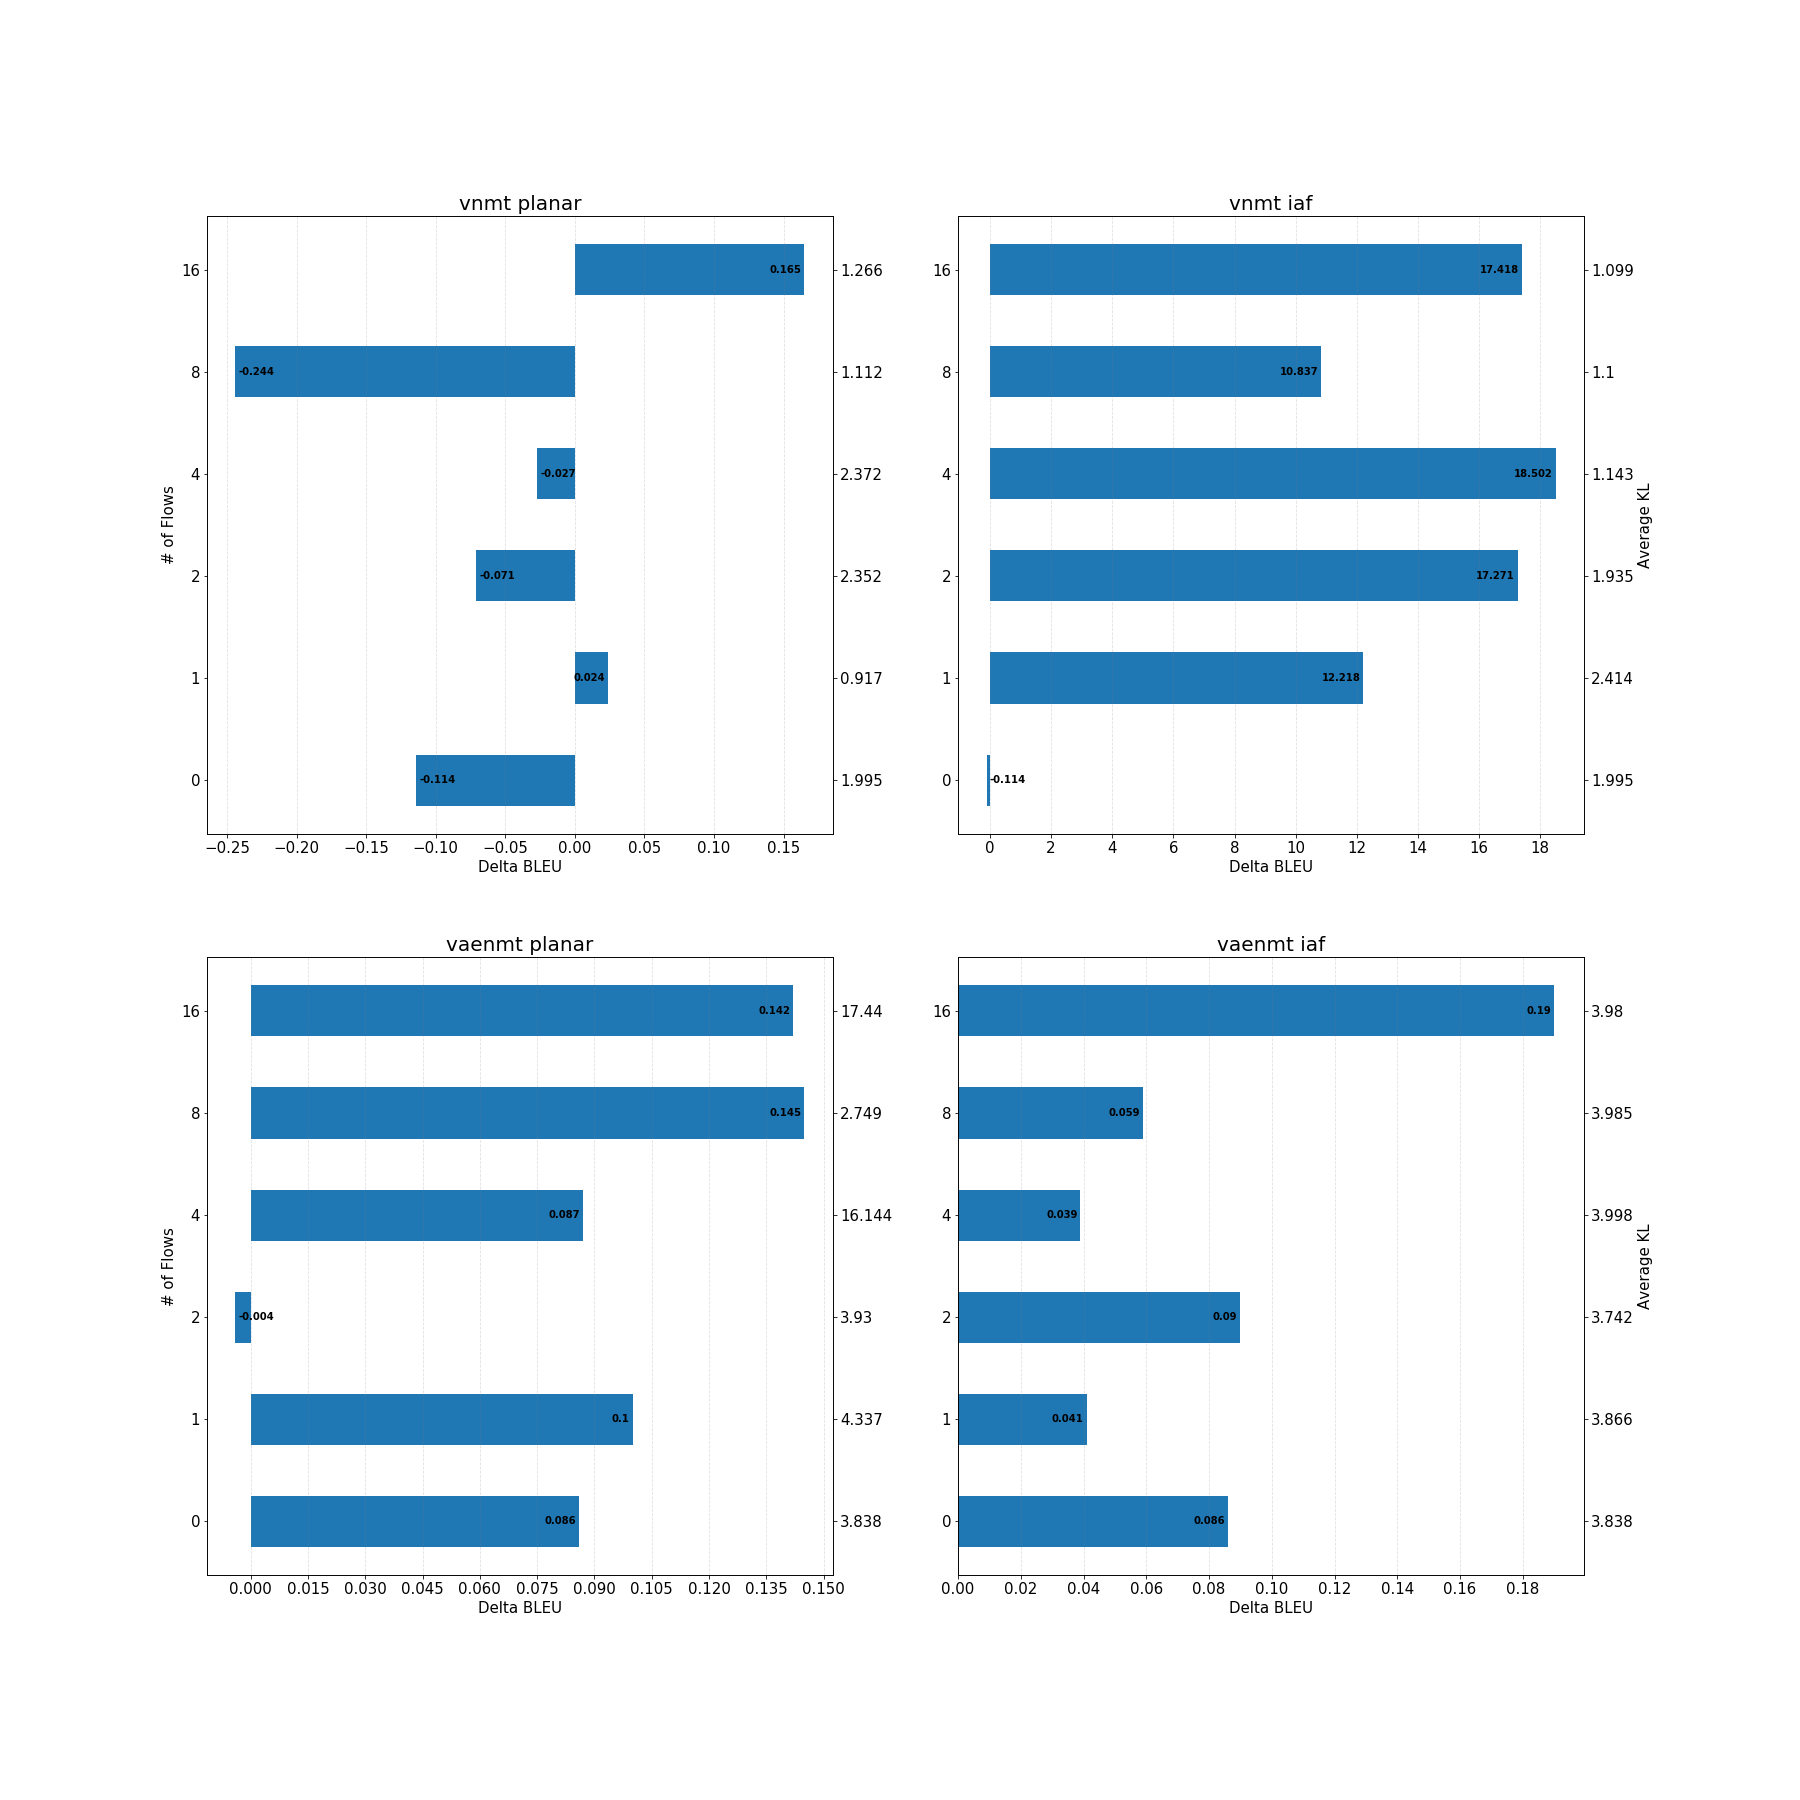
\includegraphics[width=\linewidth]{diff-z-256-horizontalbarplt.png}
	\caption{The drop in performance when we set the value of the latent variable of Z to 0 during evaluation for latent dimensions set to 256. Bars are $BLEU_{Z=\mu} - BLEU_{Z=0}$. KL divergence of model is included on right axis, number of flows on left axis.}
	\label{fig:barperfdrop}
\end{figure}

\section{Language Modelling Performance}

Hypothesis: Including normalizing flows improve the performance of the language model learned as part of the generative machine translation system. [This is related to a SPECIFIC model and is not applicable to the discriminative version of this stuff...just want to make sure that's clear]
As previously discussed in chapter 3, the generative machine translation system is trained with a language model component as part of the optimization process. In this section, we look at how the performance of this component is affected by the inclusion of normalizing flows by evaluating the performance of the learned language model during the training procedure. We measure the BLEU score and perplexity  [ are there other metrics I should consider?] for the generated source side sentences in our GNMT model. Note that the -ELBO in [Fig of ELBO] is already reported as this module is learned along with the translation system.

for Language model:
Intrinsic metric: generate sequence that is expected: Lower the better (evaluating itself against...itself? you can evaluate. Use perplexity => method of identifying how close the model will predict a given sequence. How close to the language model it was trained on. 

perplexity is sitll for the language model performance

Extrinsic evaluation: Put your language model into something else. e.g. plug into MT system, does it help machine translation?
How do we know if it helped or not? did bleu score go up or not? 
does the effect adding the language model vs adding flows
4 settings: LM + flows, LM + w/o flows, w/o LM + flows, w/o Lm model + w/o flows


extrinstic




% #make sure code is clean

%\section{Out of Domain Translation}

%We considered different data sets to do this..

\section{Understanding Latent Variable}

considerations:
\begin{enumerate}
	\item set Z = 0 vector
	\item set Z ~ N(0, 1) vector
	\item set Z swapped with nearest neighbors??
	\item Visualize latent variables from transformation
\end{enumerate}